\documentclass{article} % For LaTeX2e
\usepackage{hyperref}
\hypersetup{
   colorlinks=true,    % false: boxed links; true: colored links
   linkcolor=blue,    % color of internal links
   citecolor=blue,    % color of links to bibliography
   filecolor=blue,    % color of file links
   urlcolor=blue      % color of external links
}
\usepackage[utf8x]{inputenc}
\usepackage[T1]{fontenc}
\usepackage{nips11submit_e,times}
\usepackage{natbib}
\usepackage{amsmath}
\usepackage[pdftex]{graphicx}
\usepackage{verbatim}
%\documentstyle[nips10submit_09,times,art10]{article} % For LaTeX 2.09


\title{A Common GPU n-Dimensional Array \\
 for Python and C}


\author{
Frédéric Bastien, Arnaud Bergeron, Pascal Vincent and Yoshua Bengio \\
D\'epartement d'Informatique et de Recherche Op\'erationnelle\\
Universit\'e de Montr\'eal\\
Montr\'eal, Canada \\
\texttt{\{bastienf, bergearn, vincentp, bengioy\}@iro.umontreal.ca} \\
}

% The \author macro works with any number of authors. There are two commands
% used to separate the names and addresses of multiple authors: \And and \AND.
%
% Using \And between authors leaves it to \LaTeX{} to determine where to break
% the lines. Using \AND forces a linebreak at that point. So, if \LaTeX{}
% puts 3 of 4 authors names on the first line, and the last on the second
% line, try using \AND instead of \And before the third author name.

\newcommand{\fix}{\marginpar{FIX}}
\newcommand{\new}{\marginpar{NEW}}

\nipsfinalcopy % Uncomment for camera-ready version

\begin{document}


\maketitle

\begin{abstract}
Currently there are multiple incompatible array/matrix/n-dimensional base object implementations for GPUs. 
This hinders the sharing of GPU code and causes duplicate development work.
This paper proposes and presents a first version of a common GPU n-dimensional array (tensor) named GpuNdArray~\citep{GpuNdArray} that works with both CUDA and OpenCL.
It will be usable from Python, C, and possibly other programming languages.
\end{abstract}

\section{Introduction}
Efficient numerical vector, matrix, and tensor computations form the core of much of scientific computing.
The Python library Numpy~\citep{numpy-2007}, the de facto standard for efficient numerical computations with CPUs in Python, provides a convenient 
arbitrary-dimensional array (i.e., tensor) object with support for \emph{strides}~\footnote{
\emph{Strides} are a way to specify for each dimension in an n-dimensional array a sub-range and the number of elements to skip when going
to the next element. 
This allows to operate on a view of the data that represents, e.g. a sub-matrix, or even only odd rows of a matrix, without copying any data.
The part to view in each dimension is specified as a range of elements, with a step between each element.
This is represented by a slice with an inclusive start index, an exclusive end index and a step.
}
and \emph{broadcasting}~\footnote{
\emph{Broadcasting} is a generalization of element-wise operations on tensors that extends certain dimensions to fit the required shape.
For example, this allows adding a vector to all columns of a matrix.
Few current GPU array implementations support this very useful construct.
It is however easy to add when we have strides support.
}.
By contrast there are at least 4 different GPU array implementations in
Python: CudaNdarray (Theano)~\citep{bergstra+al:2010-scipy},
GPUArray (PyCUDA)~\citep{kloeckner_pycuda_2009},
GPUArray (PyOpenCL)~\citep{kloeckner_pycuda_2009} and
CUDAMatrix (cudamat)~\citep{cudamat-TR2009}.
There are also other implementations like Thrust~\citep{Thrust} in C++.
One problem is that they are incompatible with each other.
Each of them implements a different subset of the features that Numpy provides on the CPU.
Some implementations support only vectors or matrices, some support only \emph{float32}~\footnote{
\emph{float32} corresponds to single precision floating point numbers.
}, or only contiguous memory layouts (no strides), etc$\ldots$
None of them targets simultaneously CUDA and OpenCL back-ends.

Our objective was to design a more flexible common GPU n-dimensional array object, 
without the limitations of current implementations, and with the hope that it may become largely adopted. 
Our specific goals for this design were to:

\begin{itemize}
\item Make a n-dimensional array base object on the GPU that supports \emph{strides} and \emph{broadcasting},
\item Have a Python interface similar to numpy.ndarray (to make it more seamless and appealing to the Python community),
\item Make the development of efficient specialized operations with this n-dimensional array no harder than with more restricted array objects,
\item Have the base object in C to allow collaboration with other non-Python projects (so that people from C, C++, Ruby, R, etc... may use the same low-level base GPU ndarray),
\item Be compatible with CUDA and OpenCL.
\end{itemize}

We believe that an arbitrary-dimensional array is a basic GPU object and that a common implementation is required.
Lacking such a basic object, programmers face added complexity when dealing with algorithms that need more dimensions than what is provided.
Having the base object support n-dimensions eliminates this complexity.
We believe that there are several reasons why there has not yet been a common GPU implementation fulfilling our objectives.

One reason may be that such a general tensor implementation on GPU is difficult and time consuming to get right and efficient.
In addition, developing an efficient operation for the general memory layout can be cumbersome or sometimes even impossible.
This can be alleviated by providing functions to convert any tensor to a desired, possibly more restricted, memory layout (such as contiguous memory).
These can then be used to convert the inputs for kernels that support only a certain restricted layout.

Another reason may be that support for additional dimensions requires extra computations for index computation in the kernel which can sometimes outweigh the useful computation performed on the GPU.
In order to offset this cost, automatic optimizations like the collapsing of dimensions can be done before launching the kernel.  
This is currently implemented for element-wise operations as discussed in section~\ref{sec:currentimpl}.

We believe that if we provide such optimized functions for element-wise and reduction operations, we will cover enough cases where the conversion from one memory layout to another can be combined with computations.
\footnote{This can still impact the performance due to coalescing constraints (the hardware has different speeds for different memory access patterns), but we don't expect that to be significant, most of the time.}

\section{Existing GPU array implementations}
\subsection{Theano}
Theano is the system that provides the closest approximation of a GPU tensor. 
According to its web site Theano~\citep{bergstra+al:2010-scipy} is: ``a Python library that allows you to define, optimize, and evaluate mathematical expressions involving multi-dimensional arrays efficiently''.

It implements a GPU tensor with strides and broadcasting, but supports only float32 and the CUDA back-end.
Also, the strides information are stored differently than in numpy.
Theano stores the number of elements to skip to access the next element while numpy stores the number of bytes to skip.

\subsection{PyCUDA/PyOpenCL}
PyCUDA~\citep{kloeckner_pycuda_2009} and PyOpenCL~\citep{kloeckner_pycuda_2009} are Python wrappers around CUDA and OpenCL respectively.
In addition to wrapping their respective library, they do automatic memory management, provide a GPUArray object and some abstraction for compilation.
They also automatically translate errors to Python exceptions.

Their GPU array objects are limited to contiguous memory regions.
They add shape properties to allow using this contiguous memory region as n-dimensional array.
They don't support strides nor broadcasting, but they support many data types other than float32.

\subsection{CUDAMat}
On the CUDAMat~\citep{cudamat-TR2009} website we find the following mission statement: ``The aim of the cudamat[sic] project is to make it easy to perform basic matrix calculations on CUDA-enabled GPUs from Python. cudamat provides a Python matrix class that performs calculations on a GPU.''

So it supports only CUDA and matrices. 
If we look deeper we see that it doesn't support strides and supports only float32. 
Broadcasting is supported via a function, but not via the usual numpy syntax.

\subsection{Gnumpy}
Gnumpy~\citep{gnumpy-TR2010} is built on top of CUDAMat.
It works only with contiguous n-dimensional arrays and does not support strides.
It also adds support for the boolean type by using 1.0 and 0.0 in floating point to represent true and false, respectively. 
It also supports broadcasting via the numpy syntax.

\subsection{Thrust}
Thrust~\citep{Thrust} is a C++ template library.
It provides a vector object for CUDA.
It supports all data types, but only one dimensional vectors.
This means no broadcasting and no strides.

\subsection{Summary regarding existing implementations}
We see clearly that none of these implementations offer all of what we would like for a flexible numpy-like common GPU tensor.
As the Theano implementation supports strides and that it is easier to add other types than to add stride support, we used its code as a starting point for our implementation.
Theano also implements some optimizations of indexing computations to lower the performance cost of having more dimensions.

\section{Current state of our common GPU array implementation}
\label{sec:currentimpl}
We currently have all the code implemented and working for CUDA.
The OpenCL implementation is only missing the copy of non-contiguous memory regions.

\subsection{Functionality}

The current base code can allocate arrays, transfer data to and from the CPU, create views of that data (such as sub-arrays with strides) and run element-wise kernels with dimensions collapsing.
In order to support multiple back-ends (CUDA, OpenCL, ...) we have created a list of utility functions that are to be implemented for each 
while the rest of the code is shared.

The back-end independent parts take care of indexing, making views, and provide an interface that is very similar to numpy.
This is the part that supports any (valid) combination of dimensions and strides.
Most importantly, the dimension collapsing optimizations are device-independent and can be reused between back-ends.

We started the implementation of sum reductions in CUDA.
We have done reductions over all axis or over 1 axis when the input have 1, 2 or 3 dimensions after dimension collapsing.

We are still missing some fonctionalities before we reach full numpy compatibility, most importantly setting a part of the array via assignation and reshaping.

\subsection{Element-wise dimensions collapsing}

To lower the indexing computation cost incurred with the increasing number of dimensions, we can try to \emph{collapse} consecutive dimensions for the purpose of doing element-wise computations.
For example, if we add tensors that are both C-contiguous (row-major) or f-contiguous (column-major), we can use the same kernel for all dimensions (effectively collapsing any number of dimensions to one) since the result will be the same.
This way,  we avoid most of the index computations.

In general, any non-strided dimension can be collapsed leaving only the index for the strided dimensions to be computed in the kernel.
So if we have only the last dimension of a tensor that has strides, then we can collapse all the other dimensions (assuming that the other inputs don't have strides) and only do the indexing computations for one collapsed dimension and the original strided one.

\section{Benchmarks}

In order to measure the overhead of indexing computations relative to existing implementations, we compared two element-wise kernels generated with PyCUDA to some generated using our algorithm (including dimension collapsing and data with strides).
The timings shown below do not include transfer time nor allocation of output.
They were measured on a GeForce GTX 580.

We can conclude from these benchmarks that we have a bigger base computational cost than PyCUDA, but that this base cost is not significant when the number of elements is large.
We can see the speedup that is brought by the dimension collapsing by comparing the "GPU ndarray 4d contiguous" and "GPU ndarray 4d contiguous not collapsed" lines.

Normally on the GPU, one would expect strided access to be slower.
However "GPU ndarray 4d strided outer" (collapsed to 2 dimensions, with strides) is significantly faster then "GPU ndarray 4d contiguous not collapsed" (4 dimensions without strides).
In this case we see that strides computation has a lower overhead than uncollapsed plain indexing.
There are other optimizations that we could use to lower the index computation cost, for example we could use the implicit loops in CUDA/OpenCL.


\section{Future Plans}

We plan to continue lowering the overhead paid for the added flexibility of having strides and arbitrary dimensions 
as much as possible and to complete the OpenCL implementation.
We also plan to implement reduction operations and to contact people from the C/C++ community to have a good interface available in that language.
We will also make element-wise code use the implicit looping available in CUDA and OpenCL.

Since some Theano authors are working on this project, it will see some usage in a future version. PyCUDA and PyOpenCL, on their side, have already started a branch to use this new object.

%\hspace{-2cm}
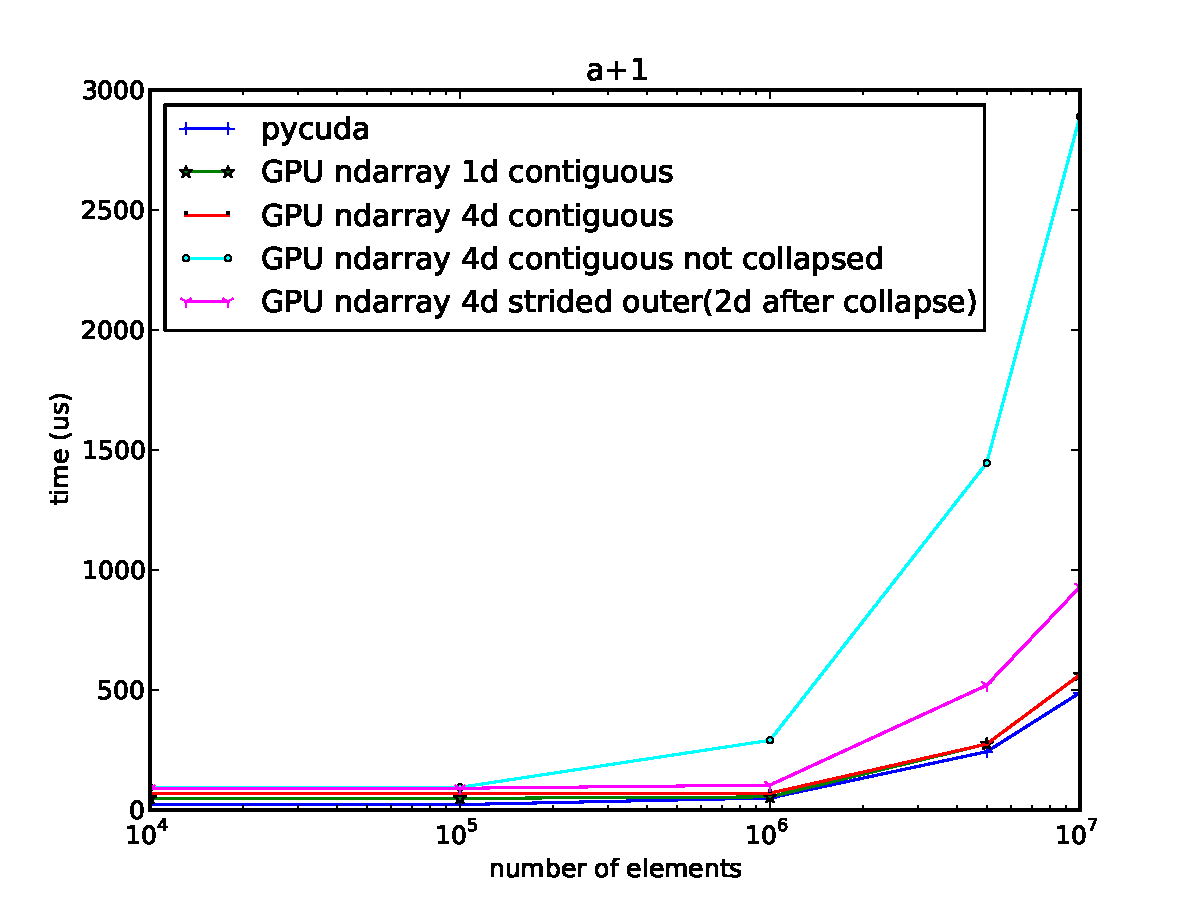
\includegraphics[width=0.85\textwidth]{ap1_no_alloc}

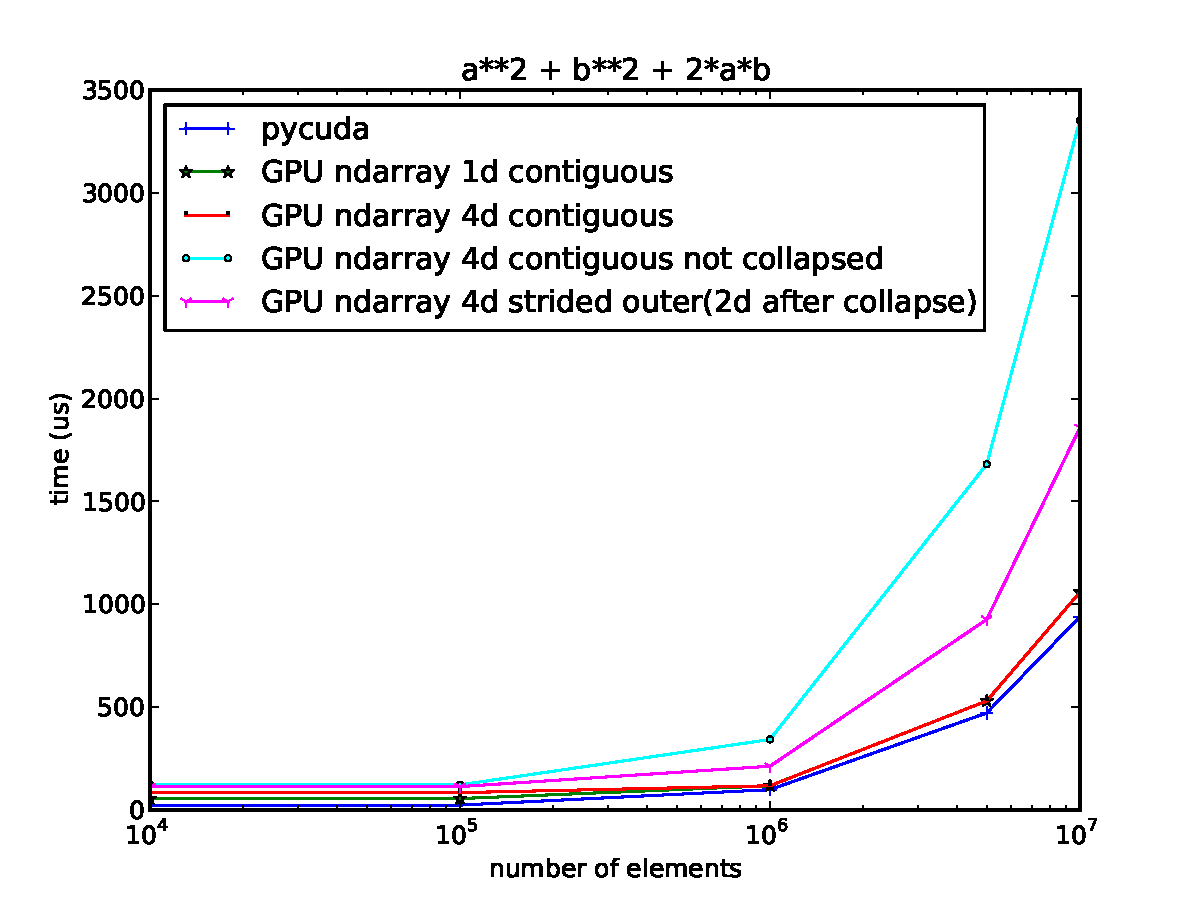
\includegraphics[width=0.75\textwidth]{a2pb2p2ab_no_alloc}


\section{Conclusion}

We have motivated the need for a more general and flexible common GPU n-dimensional array, with a similar level of functionality than Numpy's ndarray.
Our implementation shows that it is possible to work around the additional complexity with the help of functions that convert memory layouts and automatic optimization techniques like collapsing dimensions.
We hope that people can appreciate the potential benefits that such a common GPU array object would provide and will consider this project for their future numerical computation needs.

\subsubsection*{Acknowledgments}

We want to thank James Bergstra. We used some of his code as the first version of some of the functionalities currently implemented. We thank Andreas Kloeckner for his support and useful discussions. We would also like to acknowledge Compute Canada, RQCHP, NSERC, and Canada Research Chairs for providing funds or access to compute resources.


\bibliography{strings,strings-shorter,ml,aigaion-shorter}
\bibliographystyle{plain}

\end{document}
